\subsubsection{Diferencia de frecuencias absolutas}
Como bien apuntan \cite{monroe2008fightin}, esta comparaci\'on no resulta tan rica
a la hora de contrastar lemas empleados por los distintos conjuntos de
votantes puesto que se ve fuertemente influenciada por la cantidad y longitud
de los discursos emitidos por cada grupo.
\par
En nuestro caso, se observa que la mayor\'ia de los lemas son caracter\'isticos
del grupo de los votantes positivos, pero esto es una consecuencia del hecho
de que es el conjunto de estos votantes precisamente el que mayor cantidad de
discursos emiti\'o, as\'i como tambi\'en, de mayor longitud, como muestra la distribuci\'on
de la figura \ref{fig-distrib-unique-tokens}. Asimismo, vemos en la figura
\ref{fig-statistics-freq-abs} que las palabras identificadas como caracter\'isticas
de cada grupo (las azules, de los votantes a favor y las rojas, de los votantes
en contra) no resultan significativas puesto que la mayor\'ia de ellas constituyen
palabras con escaso o nulo significado sem\'antico (son verbos como `tener' o
determinantes, como `el' o `la'). Esto se evidencia sobre todo en el caso de
los votantes a favor.

\begin{figure}[h!]
    \centering
    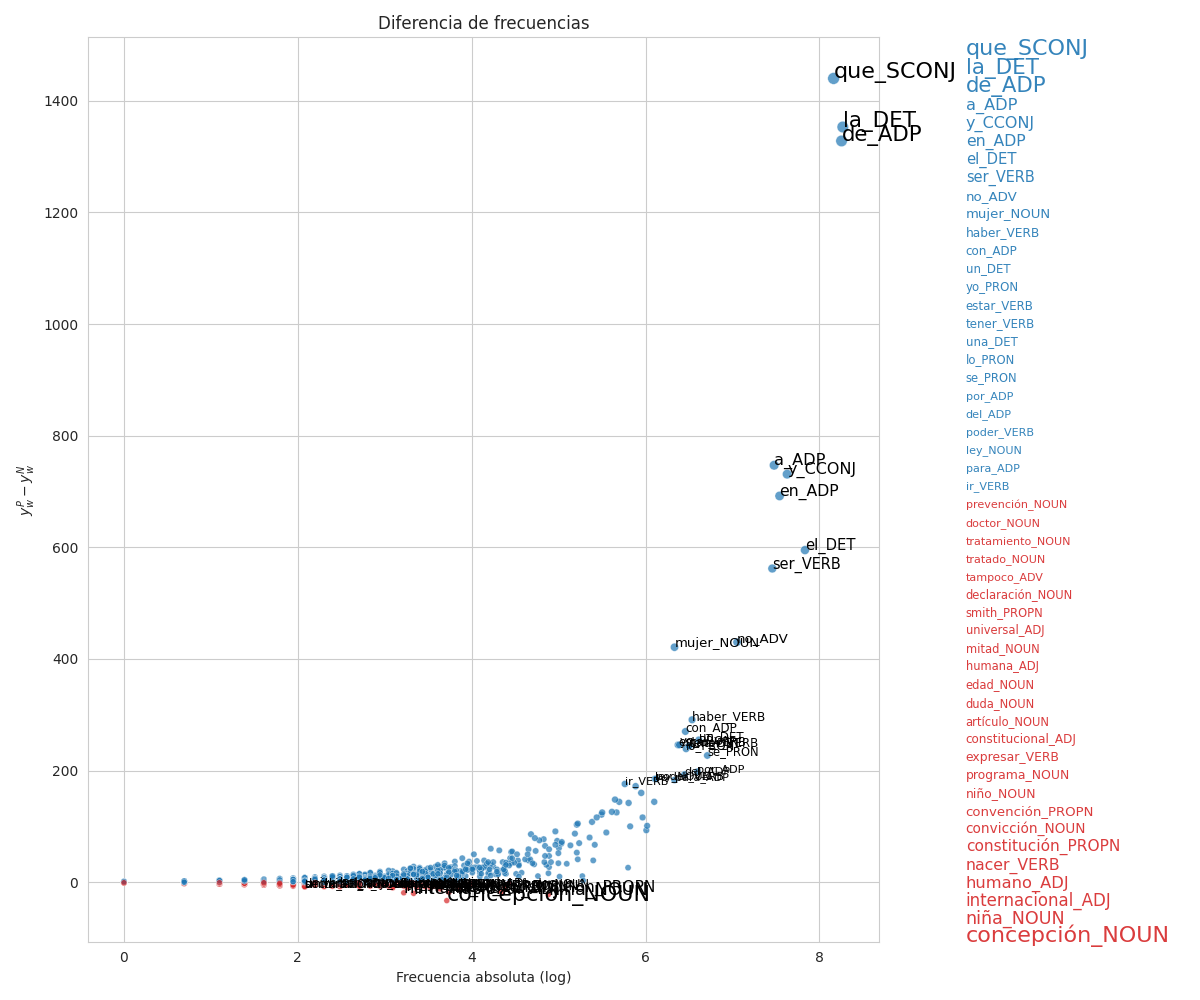
\includegraphics[scale=0.4]{../visualizations/stats/frecuencias.png}
    \caption{Comparaci\'on de palabras caracter\'isticas de los votos afirmativos y
    negativos tomando como medida la diferencia de frecuencias absolutas descripta
    en la secci\'on \ref{subsubsec-methods-freq-abs}. El eje de abscisas indica el
    logaritmo de la frecuencia absoluta de cada palabra en el conjunto de total
    de discursos y el eje de ordenadas, la comparaci\'on en cuesti\'on. En la
    columna de la derecha se observan las 25 palabras m\'as representativas de
    cada grupo de votantes escaladas seg\'un su relevancia.}
    \label{fig-statistics-freq-abs}
\end{figure}

Entre las 25 palabras m\'as caracter\'isticas del grupo de votantes positivos
encontramos mayormente determinantes (`la', `el', `un'), pronombres 
(`yo', `lo', `se'), preprocisiones (`de', `a', `en') o verbos de escaso
significado sem\'antico (`ser', `haber', `estar'). La palabra m\'as relevante
para la tem\'atica en cuesti\'on parece ser el nombre `mujer', que denota a
quien, al menos desde cierta perspectiva, es el
sujeto protagonista en el curso de un embarazo y un posible aborto. En el grupo
de votantes, sin embargo, pueden observarse una mayor cantidad de palabras
de contenido que parecen reflejar cierta
postura o cuestionamiento respecto del aborto: sobre su consitucionalidad
y su lugar en la vida de una sociedad o privada de los ciudadanos
(`civil', `constitucional'), sobre si resulta un acto moral (`mala'),
sobre qu\'e actos poner el foco (`respetar', `nacer', `concepci\'on').

\subsubsection{Diferencia de proporciones}
\label{subsubsec-results-proporcions}
Al normalizar la frecuencia absoluta de cada palabra con la cantidad
de palabras totales emitidas por cada grupo, el c\'alculo de proporciones permite
superar la limitaci\'on observada en el apartado anterior.
La figura \ref{fig-statistics-proportions} ya no muestra en su mayor\'ia palabras
vinculadas al grupo de votantes a favor de la legalizaci\'on, sino que tambi\'en
deja ver una gran cantidad de palabras relacionadas al grupo de votantes en contra.
Sin embargo, este an\'alisis sigue careciendo de validez sem\'antica puesto que, como bien
indican \cite{monroe2008fightin}, no deja de asignarle mayor peso a aquellas palabras
que ocurren con m\'as frecuencia. Si bien se observa una mayor presencia de palabras
con cierta significatividad para la tem\'atica abordada, la mayor\'ia de los lemas
que el procedimiento arroja como caracter\'isticos est\'an m\'as asociados a palabras
de uso frecuente en la lengua, m\'as que a posiciones pol\'iticas particulares. As\'i,
dentro de las palabras indicadas como representativas de los votantes a favor,
volvemos a encontrar determinantes (`la', `esa'), preprocisiones (`a', `en'),
y adverbios (`hoy', `tambi\'en'). Pero tambi\'en se encuentran nombres y verbos
de relevancia que parecen indicarnos cu\'al es el centro de la discusi\'on para el
grupo de votantes a favor de la legalizaci\'on: la mujer, el embarazo y la
de decisi\'on. Por parte del grupo de votantes negativos, similar al caso de
la diferencia de frecuencias absolutas, las palabras que resultan
caracter\'isticas parecen resaltar  el momento de la concepci\'on y el nacimiento.
Tambi\'en vuelve a aparecer cierta cuesti\'on sobre lo consitucional o sobre el derecho.
E irrumpe, como novedad, la palabra `vida'.

\begin{figure}[h!]
    \centering
    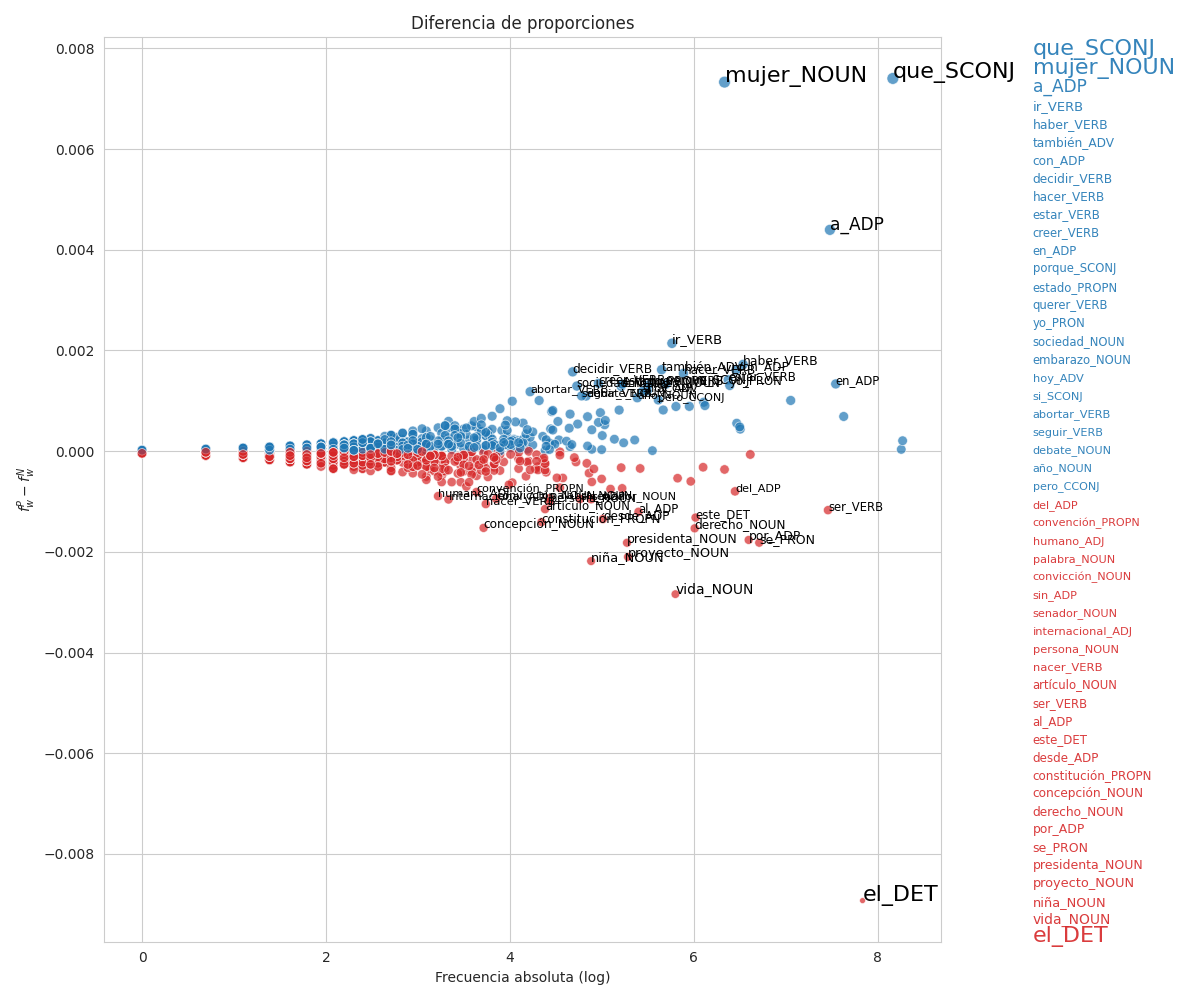
\includegraphics[scale=0.4]{../visualizations/stats/proporciones.png}
    \caption{Comparaci\'on de palabras caracter\'isticas de los votos afirmativos y
    negativos tomando como medida la diferencia de proporciones descripta
    en la secci\'on \ref{subsubsec-methods-proportions}.}
    \label{fig-statistics-proportions}
\end{figure}

\paragraph{Correcci\'on: remoci\'on de \textit{stopwords}}
\cite{monroe2008fightin} señalan que, si bien numerosos abordajes proponen remover
las palabras consideradas \textit{stopwords} del \textit{corpus} a analizar con el
fin de no viciar m\'etricas como el c\'alculo de proporciones, ellos consideran inapropiado
emplear tales metodolog\'ias puesto que es posible que, en tal remoci\'on, se acaben
eliminando tambi\'en palabras de inter\'es para el estudio en cuesti\'on. En este caso,
palabras como `ella' podr\'ian ser eliminadas cuando resultan sumamente relevantes
puesto que quienes atraviesan un embarazo y, potencialmente, la necesidad de un
aborto, son mujeres, por lo que la presencia de tales vocablos en el discurso, sumado
a otras palabras, puede indicar cierto posicionamiento. Con el objectivo de
contrastar lo sostenido por los autores, aqu\'i se intentaron dos remociones empleando
distingos m\'etodos para la definici\'on del conjunto de \textit{stopwords}.

\subparagraph{Librer\'ia NLTK}
Como se adelant\'o en \ref{subsubsec-methods-proportions}, se tom\'o el conjunto cerrado de
\textit{stopwords} predefinido por esta librer\'ia y se removi\'o tales ocurrencias
del corpus trabajado.
Luego se volvi\'o a realizar el an\'alisis de proporciones y, esta
vez, se observ\'o una menor cantidad de palabras funcionales,
como preposiciones o determinantes, dado que suelen ser estas
las palabras catalogadas como \textit{stopwords} en la mayor\'ia de
los \textit{corpora} prefefinidos. Y, una vez m\'as, apreciamos palabras que indicar\'ian
cierto foco del debate en la mujer, la decisi\'on, la autonom\'ia y la posibilidad de
interrupci\'on. Emerge un nuevo concepto, como el de la clandestinidad, y tambi\'en
el de gestante, que permite describir a la persona que atraviesa un embarazo por
su condici\'on transitoria antes que por su identida de g\'enero o, incluso, su
sexualidad.
En cuanto a los discursos que se pronunciaron en contra, volvemos a
encontrar una fuerte presencia de lemas vinculados al deber, el derecho
el respeto, entre otros que parecen referir al marco legal que rige una
sociedad. Del mismo modo, se vuelven a hallar como tem\'aticas el nacimiento,
la concepci\'on y la vida.

\subparagraph{Ley se Zipf}
Para la selecci\'on de \textit{stopwords} utilizando el an\'alisis de la Ley de Zipf,
se ordenaron las palabras seg\'un su frecuencia de manera decreciente y se estableci\'o
un umbral: las palabras ubicadas por encima de este umbral en el \textit{ranking}
se consideraron \textit{stopwords} debido a consituyen palabras de uso m\'as
frecunete en el \textit{corpur} y, por tal motivo, fueron removidas.
Esto llev\'o a la remoci\'on de las primeras cien palabras m\'as frecuentes, entre 
las cuales, la mayor\'ia forma parte de palabras funcionales.
Los pocos casos que no responden a esta caracter\'istica son palabras pasibles de
ser consideradas de uso frecuente en el g\'enero discursivo propio del debate pol\'itico
y de esta tem\'atica en cuesti\'on, como `aborto' y `vida'.
En el ap\'endice \ref{appendix-plots-zipf-law} podemos ver el gr\'afico que contrasta
las frecuencias de las palabras y su orden en el \textit{ranking}.
Luego de extraer el conjunto de palabras seleccionado, se procedi\'o a realizar el
mismo an\'alisis de proporciones detallado en este apartado. Nuevamente, entre
los discursos a favor, se observaron palabras relacionadas con la decisi\'on, aunque
esta vez aparecieron nuevos t\'erminos, como `voluntaria', `elegir'. Se hace presente
tambi\'en la cuesti\'on de la regulaci\'on (`legal', `justicia', `clandestinidad') y
surgen nuevos t\'erminos como `ella', `morir', `cuerpo', `igualdad'.\todo{esto se retoma despu\'es?}
Por parte de los discursos en contra, volvemos a encontrar vocablos relacionados
con la normatividad (`constitucional', `c\'odigo', `convenci\'on', `cumplir', 
`acuerdo', `tratado') y, una vez m\'as, se presentan t\'erminos relacionados
con la concepci\'on y el nacimiento.

\begin{figure}[h!]
    \centering
    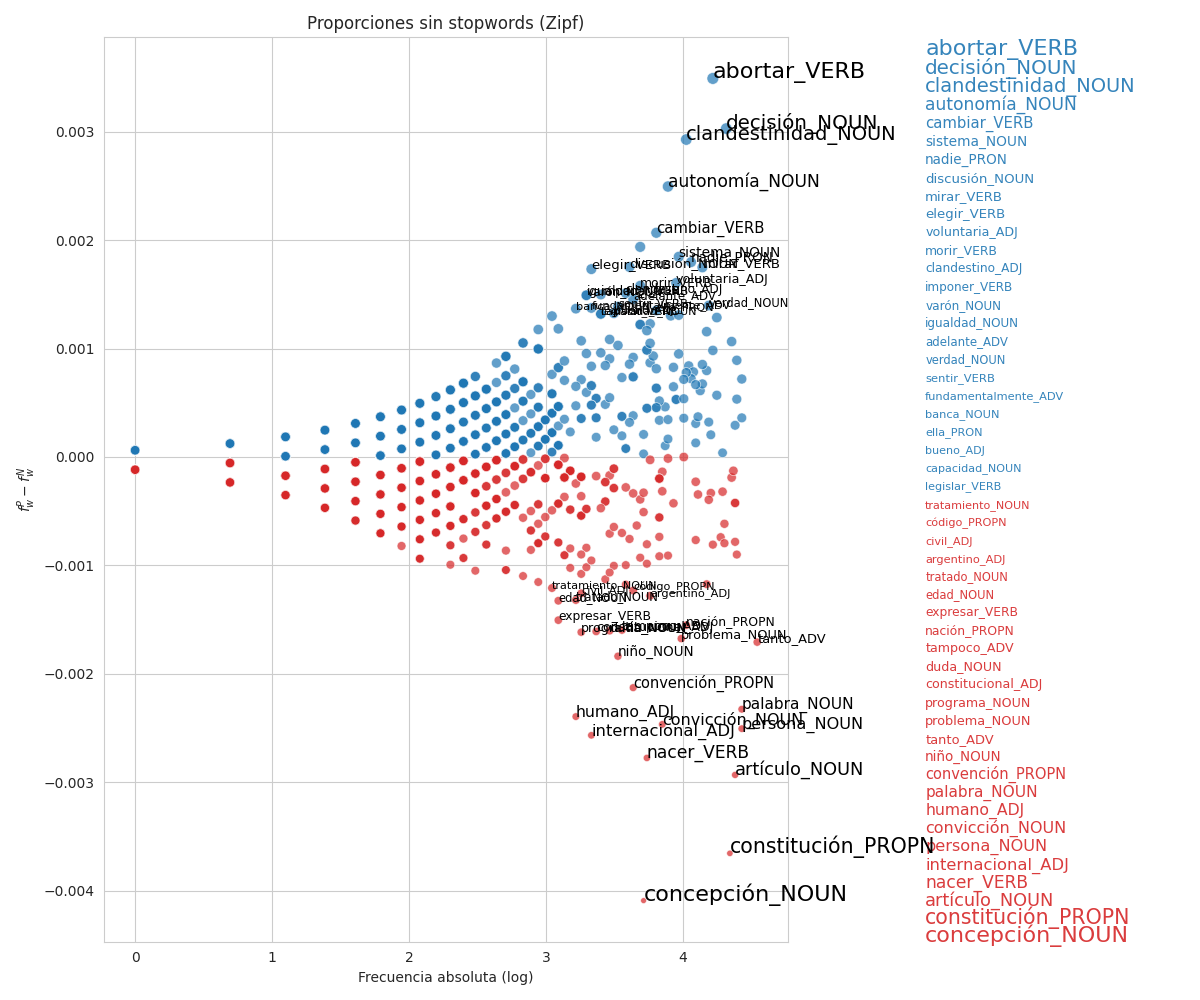
\includegraphics[scale=0.4]{../visualizations/stats/proporciones_sin_stopwords_zipf.png}
    \caption{Comparaci\'on de palabras caracter\'isticas de los votos afirmativos y
    negativos tomando como medida la diferencia de proporciones descripta
    en la secci\'on \ref{subsubsec-methods-proportions} luego de la remoci\'on de
    \textit{stopwrods} utilizando la Ley de Zipf.}
    \label{fig-statistics-proportions-zipf}
\end{figure}

\subsubsection{Ratio de \textit{Odds}}
A diferencia de los casos anteriores, por la definici\'on de la funci\'on de
\textit{ratio} de \textit{odds}, el punto de corte para considerar
a una palabra como caracter\'istica de cada discurso ya no es el $0$ sino el $1$:
las palabras por encima de ese umbral ser\'an las positivas y aquellas por debajo,
las negativas. N\'otese que, dado que la ocurrencia de una palabra nunca es negativa,
los \textit{ratios} calculados solo arrojar\'an valores positivos. Por otro lado,
la funci\'on no estar\'a definida para los casos en los cuales una palabra se
observe solamente en el conjunto de discursos a favor, dado que no es posible
dividir por $0$. Se observaron 1871 registros en esta situaci\'on, todos ellos
pertenecientes a palabras presentes en los dicursos positivos y ausentes En
los negativos.
\par
Al analizar las palabras arrojadas como representativas de cada discurso, se
encuentra que el grupo de votantes a favor hace referencia a las violaciones
(con el adjetivo `violada'); a la clandestinidad (con el adjetivo `clandestina'),
y a la interrupci\'on legal del embarazo (con la sigla `ILE'). Vuelve a aparecer,
a su vez, la cuesti\'on de la elecci\'on (con el verbo `elegir'), y hallamos tambi\'en
la presencia de verbos referentes al castigo (`castigar'), al parto (`parir') y
al hecho de juzgar. Por otro lado, en los discursos negativos se encontraron
adjetivos como `inoportuno'; sustantivos como `respaldo', `juicio' y `hambre', 
y verbos como `aprovechar' y `justificar'.

\subsubsection{Ratio \textit{Log-odds}}

Los resultados de aplicar el logaritmo sobre el ratio de \textit{odds} no distaron
de los observados sin su aplicaci\'on. La \'unica mejora se dio en
t\'erminos de la visualizaci\'on de los datos: al tomar logaritmo, el umbral que separa
las palabras de los discursos positivos de los negativos vuelve a ser el $0$ y,
similar a lo que ocurre en los gr\'aficos anteriores, los puntos representativos
de las palabras se ordenan de forma espejada, mientras que, sin tomar logaritmo,
esto no ocurri\'o y la interpretabilidad de los datos result\'o m\'as dificultosa.

\paragraph{Suavizado}
As\'i como ocurr\'ia con el ratio de \textit{odds}, el ratio de \textit{log-odds} no
permite capturar claramente aquellos csos en los que una palabra solo se observa en
un grupo de discursos pero no en el otro. Por su formulaci\'on, cuando una palabra
ocurra solamente en los discursos negativos, el logaritmo devolver\'a el valor $1$ y,
cuando solo ocurra en los discursos positivos, la funci\'on estar\'a indefinida. Para
superar esta limitaci\'on, se aplic\'o un suavizado sobre tales casos.
\par
Sin embargo, como señalan \cite{monroe2008fightin}, si bien esta t\'ecnica permite
lidiar con las palabras conf frecuencia $0$ para alg\'un grupo discursivo, arroja,
en cada caso, un conjunto de palabras cuya interepreaci\'on resulta un poco m\'as
oscura respecto de la su relevancia para el t\'opico en cuestion. En el caso
de los discursos a favor, podemos encontrar algunas m\'as claras como `m\'edica',
`matriculado', `privilegiado', entre los adjetivos, y `solvencia', entre los nombres,
pero otras menos claras como `operatividad', `tapita', `alcohol', `postre',
`desencuentro'. Y, por parte de los discursos en contra, vemos `dram\'aticp', `sordo' y
`biol\'ogico', como casos de adejtivos que podr\'ian ser m\'as f\'acilmente vinculados a la
tem\'atica, y `horizontal', `restringida', `pavada', `plasmada', `transitado', `sumado',
`ilustrar', como casos que, al menos, requieren un an\'alisis m\'as agudo para poder
aventurar una interepreaci\'on.

\subsubsection{\textit{TF-IDF}}

\paragraph{Frecuencia de documentos con logaritmo}
Similar a lo hallado por \cite{monroe2008fightin}, esta m\'etrica presenta una
fuerte correlaci\'on ($-0.96$) con los resultados arrojados por la diferencia
de proporciones. La misma es de tipo inverso debido a la naturaleza del c\'alculo
utilizado: la frecuencia relativa es simpre positiva y el logaritmo de la
frecuencia inversa de un t\'ermino en los documetnos, negativo. De modo que aqu\'i,
a diferencia de los gr\'afios anteriores, los lemas representativos de los discursos
a favor se visualizar\'an debajo del eje `x' y aquellos representativos de los
discursos en contra, por encima. Quitando esta salvedad, las palabras observadas
para cada grupo son las mismas que las detalladas en la secci\'on
\ref{subsubsec-results-proporcions} para la diferencia de proporciones.

\begin{figure}[h!]
    \centering
    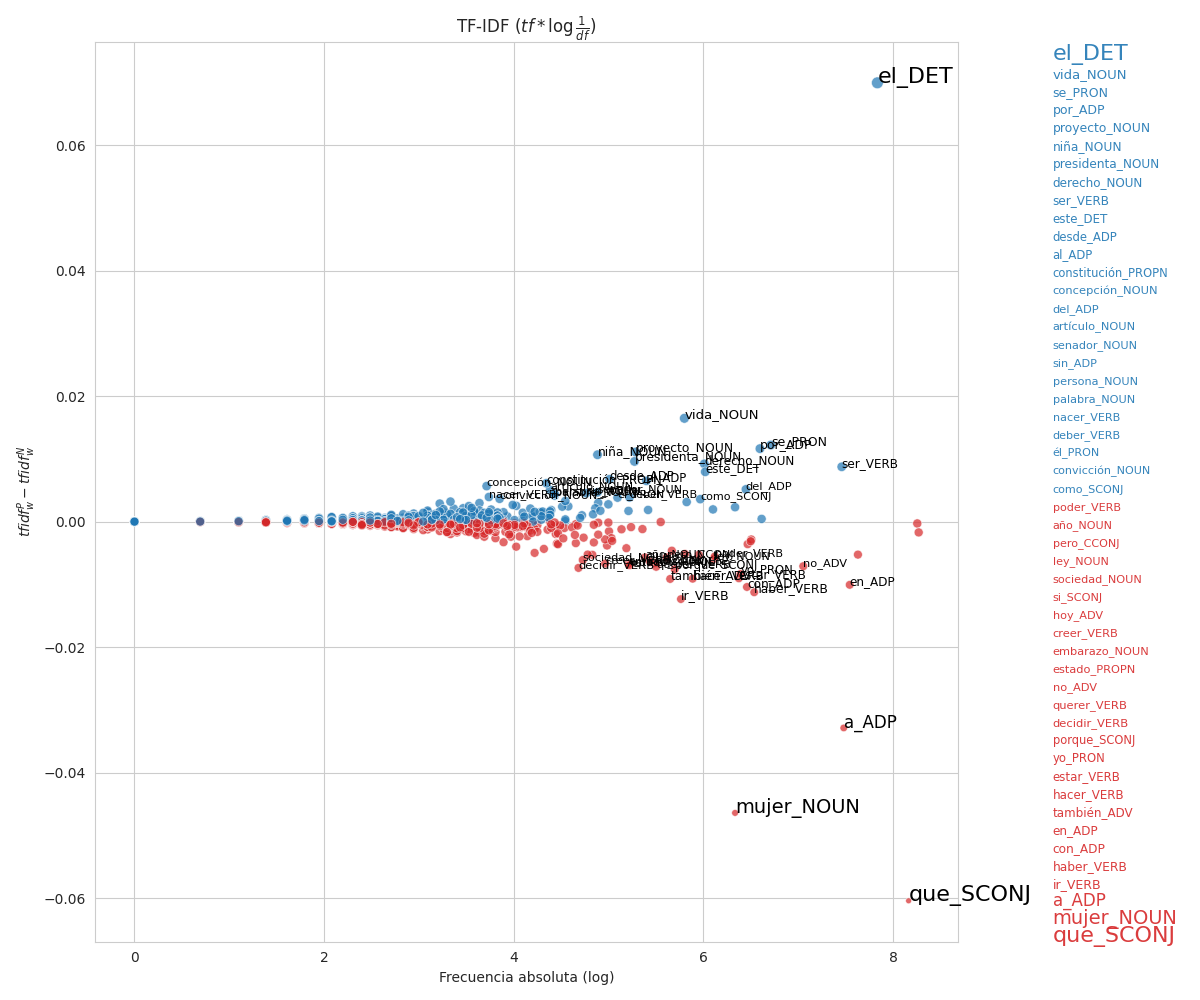
\includegraphics[scale=0.4]{../visualizations/stats/tfidf_dflogged.png}
    \caption{Comparaci\'on de palabras caracter\'isticas de los votos afirmativos y
    negativos tomando como medida \textit{TF-IDF} tomando logaritmo
    sobre \textit{IDF}, tal como se describe en la secci\'on
    \ref{subsubsec-methods-tfidf}.}
    \label{fig-statistics-wordscores}
\end{figure}


\paragraph{Frecuencia de documentos natural}
Esta m\'etrica no mostr\'o resultados de f\'acil interpretaci\'on. Las palabras de cada
grupo resultaron ampliamente variadas y con poca conexi\'on sem\'antica
entre s\'i y con la tem\'atica de inter\'es. Es por esto que, por cuestiones de espacio,
omitiremos detallarla.

\subsubsection{\textit{Word Scores}}

Tal como señalan \cite{monroe2008fightin}, en este trabajo se contata que
la m\'etrica de \textit{word scores} correlaciona fuertemente ($+0.99$) con
la calculada a partir de la diferencia de proporciones. De ah\'i que, las palabras
que arroje como caracter\'isticas de cada grupo sean las mismas que las antes
observadas. En este sentido, esta m\'etrica adolece de la misma limitaci\'on
que aquella: asigna mayor peso a palabras de uso frecuente en el discurso antes
que a aquellas que represantan mejor determinada postura.
